%%%%%%%%%%%%%%%%%%%%%%%%%%%%%%%%%%%%%%%%%
% Beamer Presentation
% LaTeX Template
% Version 2.0 (March 8, 2022)
%
% This template originates from:
% https://www.LaTeXTemplates.com
%
% Author:
% Vel (vel@latextemplates.com)
%
% License:
% CC BY-NC-SA 4.0 (https://creativecommons.org/licenses/by-nc-sa/4.0/)
%
%%%%%%%%%%%%%%%%%%%%%%%%%%%%%%%%%%%%%%%%%

%----------------------------------------------------------------------------------------
%	PACKAGES AND OTHER DOCUMENT CONFIGURATIONS
%----------------------------------------------------------------------------------------

\documentclass[
	11pt, % Set the default font size, options include: 8pt, 9pt, 10pt, 11pt, 12pt, 14pt, 17pt, 20pt
	%t, % Uncomment to vertically align all slide content to the top of the slide, rather than the default centered
	%aspectratio=169, % Uncomment to set the aspect ratio to a 16:9 ratio which matches the aspect ratio of 1080p and 4K screens and projectors
]{beamer}

\graphicspath{{Images/}{./}} % Specifies where to look for included images (trailing slash required)
\usepackage{subcaption}

\usepackage{booktabs} % Allows the use of \toprule, \midrule and \bottomrule for better rules in tables

%----------------------------------------------------------------------------------------
%	SELECT LAYOUT THEME
%----------------------------------------------------------------------------------------

% Beamer comes with a number of default layout themes which change the colors and layouts of slides. Below is a list of all themes available, uncomment each in turn to see what they look like.

%\usetheme{default}
%\usetheme{AnnArbor}
%\usetheme{Antibes}
%\usetheme{Bergen}
%\usetheme{Berkeley}
%\usetheme{Berlin}
%\usetheme{Boadilla}
%\usetheme{CambridgeUS}
%\usetheme{Copenhagen}
%\usetheme{Darmstadt}
%\usetheme{Dresden}
%\usetheme{Frankfurt}
%\usetheme{Goettingen}
%\usetheme{Hannover}
%\usetheme{Ilmenau}
%\usetheme{JuanLesPins}
%\usetheme{Luebeck}
\usetheme{Madrid}
%\usetheme{Malmoe}
%\usetheme{Marburg}
%\usetheme{Montpellier}
%\usetheme{PaloAlto}
%\usetheme{Pittsburgh}
%\usetheme{Rochester}
%\usetheme{Singapore}
%\usetheme{Szeged}
%\usetheme{Warsaw}

%----------------------------------------------------------------------------------------
%	SELECT COLOR THEME
%----------------------------------------------------------------------------------------

% Beamer comes with a number of color themes that can be applied to any layout theme to change its colors. Uncomment each of these in turn to see how they change the colors of your selected layout theme.

%\usecolortheme{albatross}
%\usecolortheme{beaver}
%\usecolortheme{beetle}
%\usecolortheme{crane}
%\usecolortheme{dolphin}
%\usecolortheme{dove}
%\usecolortheme{fly}
%\usecolortheme{lily}
%\usecolortheme{monarca}
%\usecolortheme{seagull}
%\usecolortheme{seahorse}
%\usecolortheme{spruce}
\usecolortheme{whale}
%\usecolortheme{wolverine}

%----------------------------------------------------------------------------------------
%	SELECT FONT THEME & FONTS
%----------------------------------------------------------------------------------------

% Beamer comes with several font themes to easily change the fonts used in various parts of the presentation. Review the comments beside each one to decide if you would like to use it. Note that additional options can be specified for several of these font themes, consult the beamer documentation for more information.

\usefonttheme{default} % Typeset using the default sans serif font
%\usefonttheme{serif} % Typeset using the default serif font (make sure a sans font isn't being set as the default font if you use this option!)
%\usefonttheme{structurebold} % Typeset important structure text (titles, headlines, footlines, sidebar, etc) in bold
%\usefonttheme{structureitalicserif} % Typeset important structure text (titles, headlines, footlines, sidebar, etc) in italic serif
%\usefonttheme{structuresmallcapsserif} % Typeset important structure text (titles, headlines, footlines, sidebar, etc) in small caps serif

%------------------------------------------------

%\usepackage{mathptmx} % Use the Times font for serif text
\usepackage{palatino} % Use the Palatino font for serif text

%\usepackage{helvet} % Use the Helvetica font for sans serif text
\usepackage[default]{opensans} % Use the Open Sans font for sans serif text
%\usepackage[default]{FiraSans} % Use the Fira Sans font for sans serif text
%\usepackage[default]{lato} % Use the Lato font for sans serif text

%----------------------------------------------------------------------------------------
%	SELECT INNER THEME
%----------------------------------------------------------------------------------------

% Inner themes change the styling of internal slide elements, for example: bullet points, blocks, bibliography entries, title pages, theorems, etc. Uncomment each theme in turn to see what changes it makes to your presentation.

\useinnertheme{default}
%\useinnertheme{circles}
%\useinnertheme{rectangles}
%\useinnertheme{rounded}
%\useinnertheme{inmargin}

%----------------------------------------------------------------------------------------
%	SELECT OUTER THEME
%----------------------------------------------------------------------------------------

% Outer themes change the overall layout of slides, such as: header and footer lines, sidebars and slide titles. Uncomment each theme in turn to see what changes it makes to your presentation.

%\useoutertheme{default}
%\useoutertheme{infolines}
%\useoutertheme{miniframes}
%\useoutertheme{smoothbars}
%\useoutertheme{sidebar}
%\useoutertheme{split}
%\useoutertheme{shadow}
%\useoutertheme{tree}
%\useoutertheme{smoothtree}

%\setbeamertemplate{footline} % Uncomment this line to remove the footer line in all slides
\setbeamertemplate{footline}[page number] % Uncomment this line to replace the footer line in all slides with a simple slide count

%\setbeamertemplate{navigation symbols}{} % Uncomment this line to remove the navigation symbols from the bottom of all slides

%----------------------------------------------------------------------------------------
%	PRESENTATION INFORMATION
%----------------------------------------------------------------------------------------

\title[Applying decision intelligence]{Applying decision intelligence to an industrial filtration system} % The short title in the optional parameter appears at the bottom of every slide, the full title in the main parameter is only on the title page

\subtitle{} % Presentation subtitle, remove this command if a subtitle isn't required

\author[K.C. Lewis]{K.C. Lewis} % Presenter name(s), the optional parameter can contain a shortened version to appear on the bottom of every slide, while the main parameter will appear on the title slide

%\institute[UC]{University of Cambridge \\ \smallskip \textit{james@LaTeXTemplates.com}} % Your institution, the optional parameter can be used for the institution shorthand and will appear on the bottom of every slide after author names, while the required parameter is used on the title slide and can include your email address or additional information on separate lines

\date[\today]{Johns Hopkins University Applied Physics Laboratory\\ Force Projection Sector \\ October 10, 2023} % Presentation date or conference/meeting name, the optional parameter can contain a shortened version to appear on the bottom of every slide, while the required parameter value is output to the title slide

%----------------------------------------------------------------------------------------

\begin{document}

%----------------------------------------------------------------------------------------
%	TITLE SLIDE
%----------------------------------------------------------------------------------------

\begin{frame}
	\titlepage % Output the title slide, automatically created using the text entered in the PRESENTATION INFORMATION block above
\end{frame}

%----------------------------------------------------------------------------------------
%	TABLE OF CONTENTS SLIDE
%----------------------------------------------------------------------------------------

% The table of contents outputs the sections and subsections that appear in your presentation, specified with the standard \section and \subsection commands. You may either display all sections and subsections on one slide with \tableofcontents, or display each section at a time on subsequent slides with \tableofcontents[pausesections]. The latter is useful if you want to step through each section and mention what you will discuss.

%----------------------------------------------------------------------------------------
%	PRESENTATION BODY SLIDES
%----------------------------------------------------------------------------------------

\section{Decision Intelligence} % Sections are added in order to organize your presentation into discrete blocks, all sections and subsections are automatically output to the table of contents as an overview of the talk but NOT output in the presentation as separate slides

%------------------------------------------------

\subsection{Columns}

\begin{frame}
	\frametitle{Critical Systems Thinking \cite{p1}}
	\framesubtitle{} % Optional subtitle

	\begin{columns}[c] % The "c" option specifies centered vertical alignment while the "t" option is used for top vertical alignment
		\begin{column}{0.45\textwidth} % Left column width
			\textbf{Designed to}
			\begin{enumerate}
				\item incorporate progress made in systems thinking over many decades
				\item avoid the biases of looking through just one lens
				\item leverage other approaches, such as decision intelligence, strategic options, system dynamics, etc
			\end{enumerate}
		\end{column}
		\begin{column}{0.5\textwidth} % Right column width
		    Critical Systems Thinking is a meta-framework for choosing the best combination of approaches for a given scenario
		\end{column}
	\end{columns}
\end{frame}

\subsection{Columns}

\begin{frame}
	\frametitle{Decision Intelligence \cite{p2}}
	\framesubtitle{} % Optional subtitle
	
	\begin{columns}[c] % The "c" option specifies centered vertical alignment while the "t" option is used for top vertical alignment
		\begin{column}{0.45\textwidth} % Left column width
			\textbf{Designed to}
			\begin{enumerate}
				\item enhance decision making in mission-centric scenarios
				\item avoid common pitfalls of group-based problem solving
				\item optimize use of decision assets (data mining, simulations, etc)
			\end{enumerate}
		\end{column}
		\begin{column}{0.5\textwidth} % Right column width
			We sketch an end-to-end application of Decision Intelligence, showing how it can empower decision makers by leveraging decision assets as effectively as possible.
		\end{column}
	\end{columns}
\end{frame}

%------------------------------------------------

\subsection{Paragraphs and Lists}

\begin{frame}
	\frametitle{Objective statement for a hypothetical shipping company}

	\textbf{``How can we improve the efficiency of our contaminant filtering systems?''}

	\bigskip

	\textbf{We frame the objective more precisely by answering questions such as...}

	\begin{enumerate}
	 \item who has the authority to make the decisions?
	 \item who has responsibility for the outcomes?
	 \item what are the hard constraints?
	\end{enumerate}


\end{frame}

%-------------------------------------------------------
\begin{frame}
	\frametitle{Brainstorming outcomes}

	\textbf{Putting ourselves in the decision maker's position, we could try to...}

	\begin{enumerate}
	\item reduce total cost of running the systems
	\item increase the volumetric flow rate of purified fluid
	\end{enumerate}


\end{frame}
%-------------------------------------------------------
\begin{frame}
	\frametitle{Brainstorming actions}

	\textbf{Actions that might get us to those goals:}

	\begin{enumerate}
	 \item use different filter designs
	 \item optimize maintenance
	 \item purge filters with chemical treatments
	 \item increase pressure differential to eject more biomass
	\end{enumerate}


\end{frame}
%--------------------------------------------------------

\subsection{Causal decision diagram}

\begin{frame}
    \frametitle{Causal decision diagram}
	\begin{figure}
		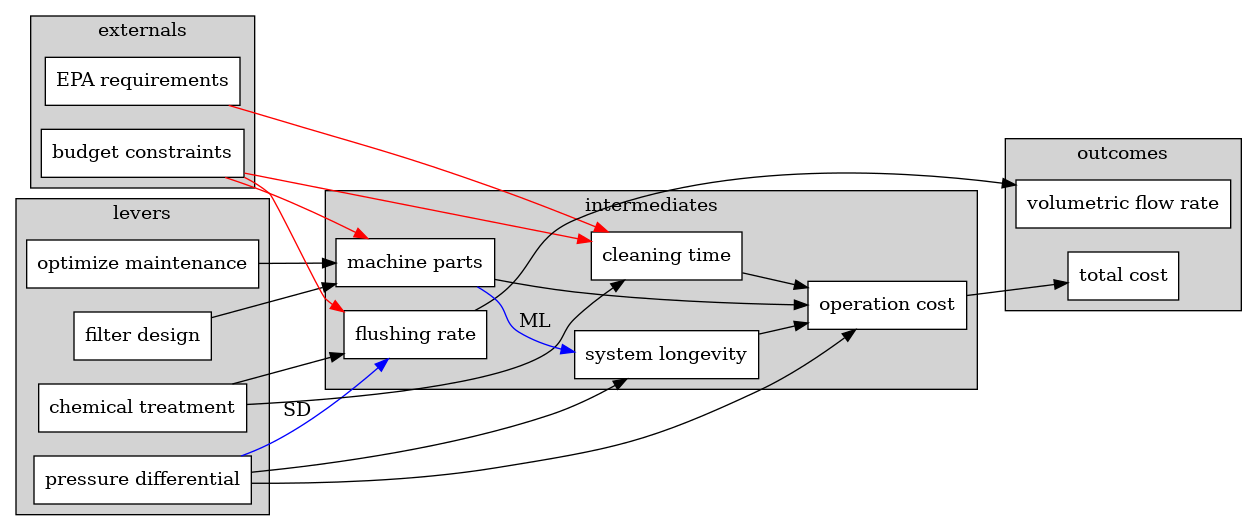
\includegraphics[width=1.0\linewidth]{causal_decision_diagram.png}
	\end{figure}
\end{frame}

%-------------------------------------------------------

\subsection{Monte Carlo simulations}

\begin{frame}
    \frametitle{Monte Carlo simulations}
	\begin{figure}
		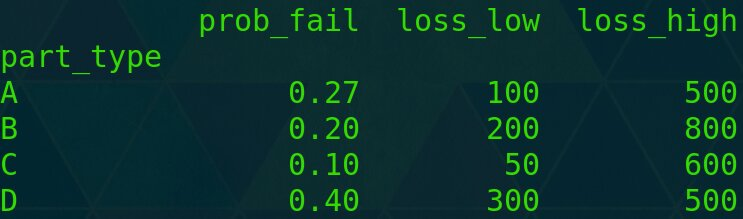
\includegraphics[width=1.0\linewidth]{machine_parts.jpg}
	\end{figure}
	\begin{figure}
	    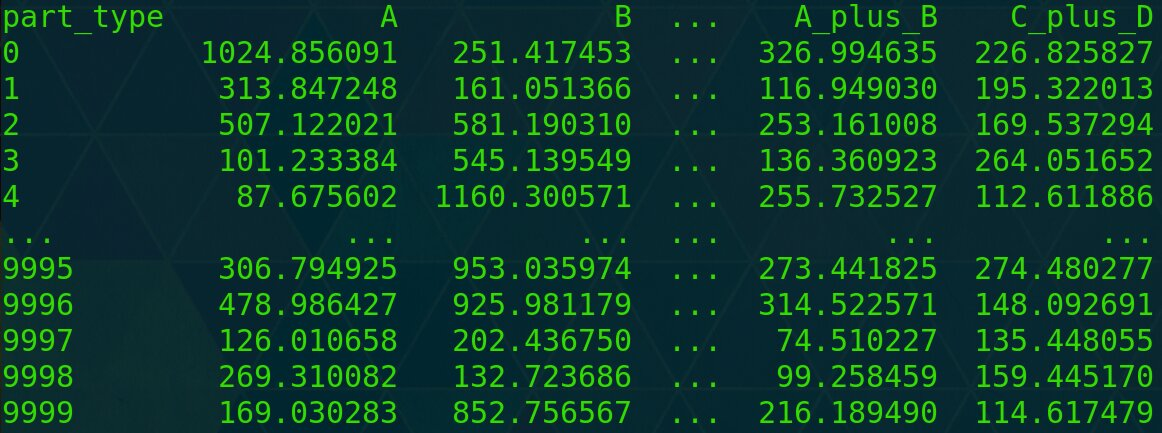
\includegraphics[width=1.0\linewidth]
	    {projected_losses.jpg}
	\end{figure}
\end{frame}

%-------------------------------------------------------

\subsection{System dynamics of biofilm detachment}

\begin{frame}
    \frametitle{System dynamics }
	\begin{figure}
		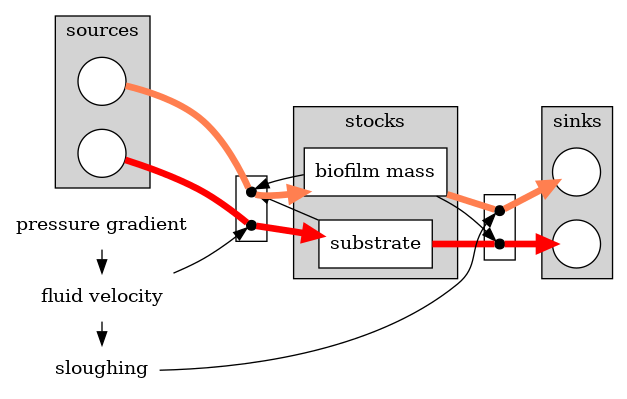
\includegraphics[width=0.7\linewidth]{system_dynamics_diagram.png}
	\end{figure}
	\vspace{-1.5cm}
	\begin{center}
	    \begin{equation*}
            \dot{M}=\alpha M + \beta CM - \gamma V
		\end{equation*}
		\begin{equation*}
            \dot{C}=\delta V - \mu MC
		\end{equation*}
    \end{center}

\end{frame}

%-------------------------------------------------------
\subsection{System vector fields}

\begin{frame}
    \frametitle{System vector field}
	\begin{figure}
		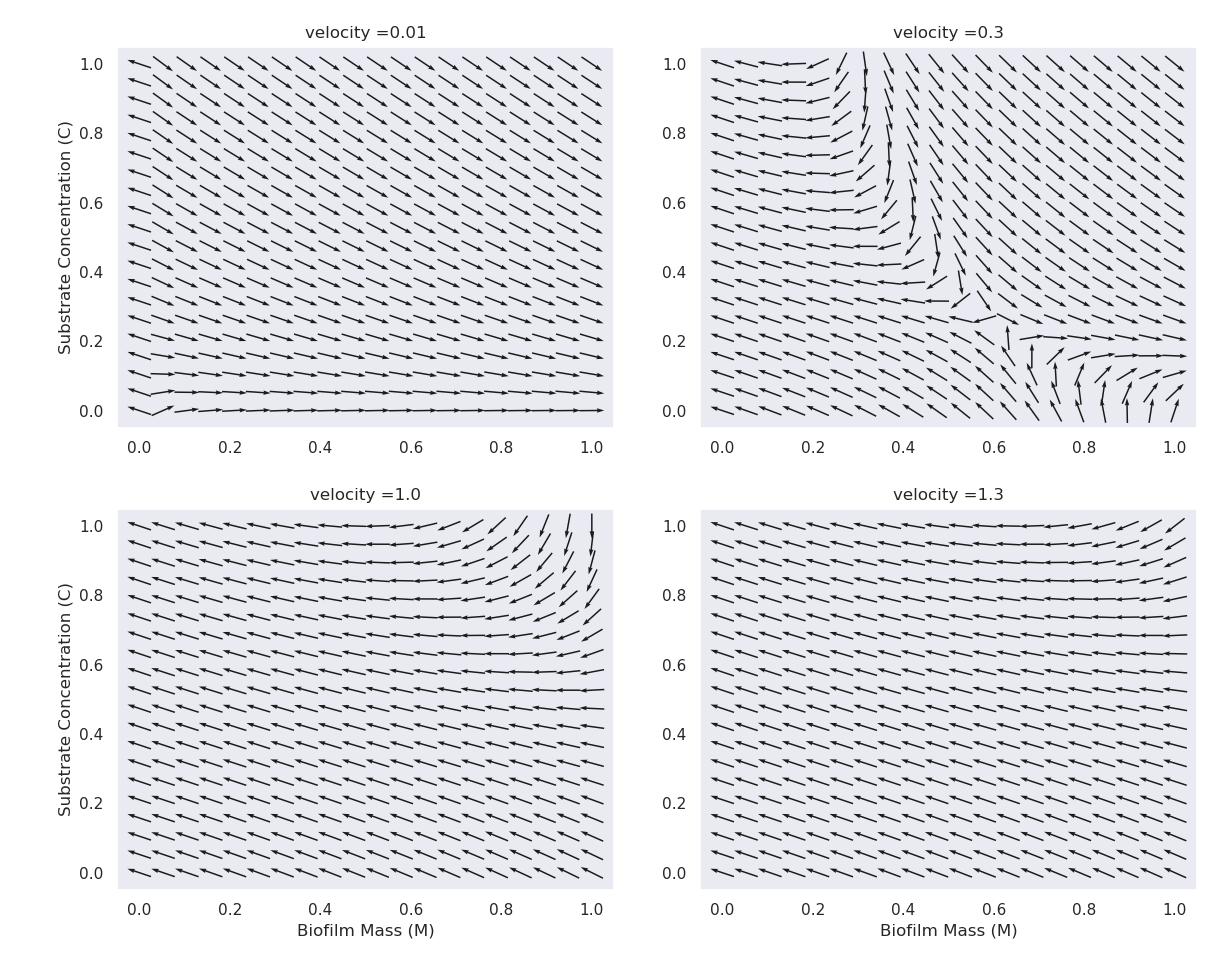
\includegraphics[width=0.8\linewidth]{system_vector_fields.png}
	\end{figure}
\end{frame}

%-------------------------------------------------------

\section{Table and Figure Examples}

\subsection{Table}

\begin{frame}
	\frametitle{Sample machine parts/maintenance data}

	\begin{table}
		\begin{tabular}{l l l l l}
			\toprule
			pump type & filter type & maintenance schedule & ... & longevity \\
			\midrule
			1 & 1 & 0 & ... & 5 \\
			0 & 1 & 1 & ... & 2 \\
			1 & 0 & 0 & ... & 5 \\
			\bottomrule
		\end{tabular}
	\end{table}
\end{frame}

%------------------------------------------------

\subsection{Figure}

\begin{frame}
	\frametitle{Decision tree classifier}
	
	\begin{figure}
		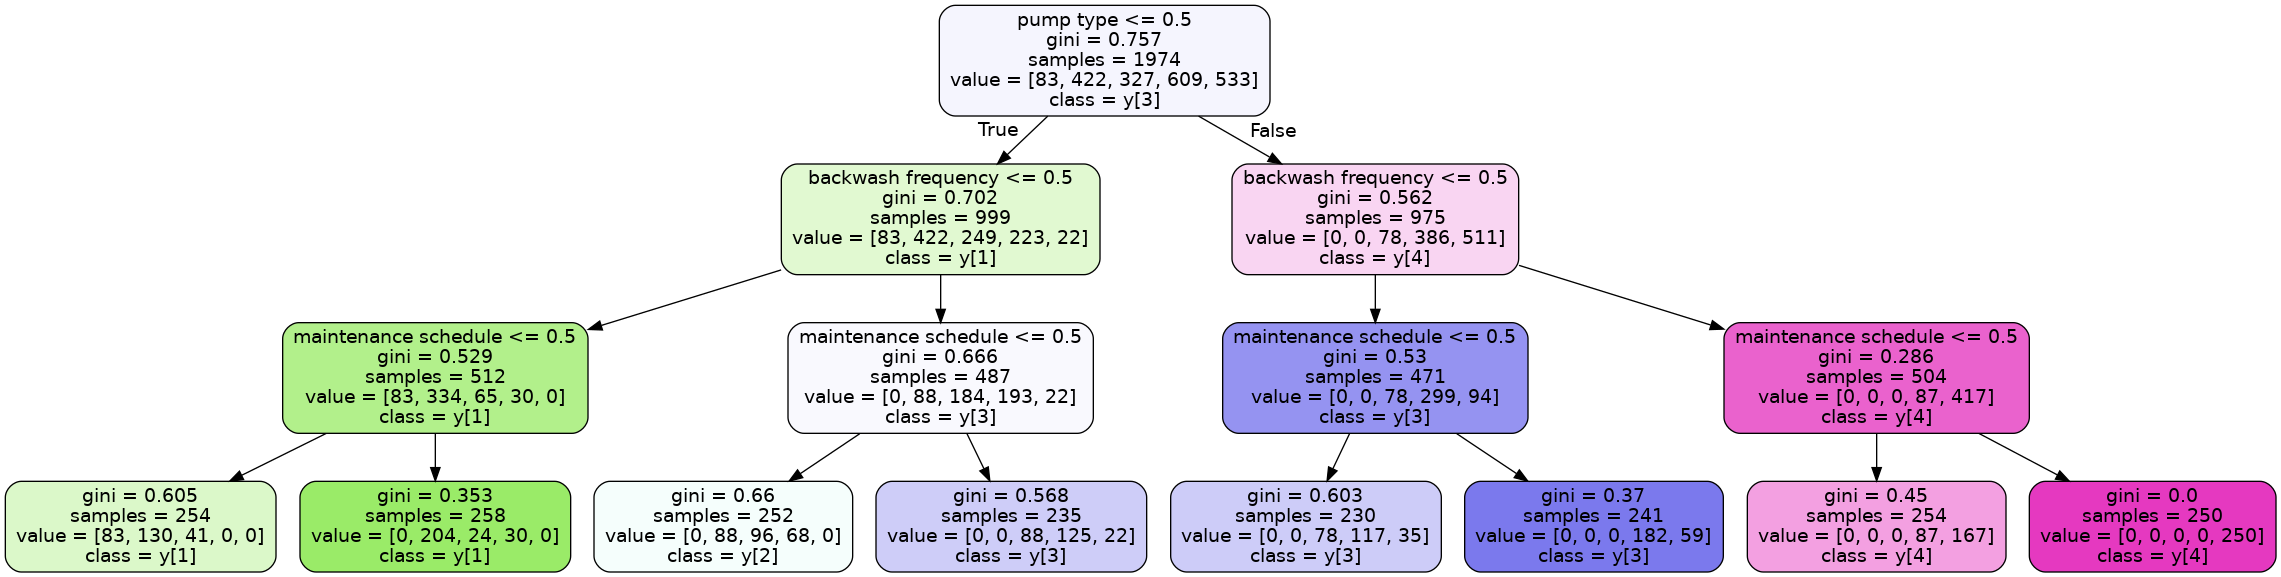
\includegraphics[width=1.0\linewidth]{decision_tree_graphviz.png}
	\end{figure}
\end{frame}

%------------------------------------------------
\subsection{Figure}

\begin{frame}
	\frametitle{How well do the models do?}

	\begin{text}
	   Both the decision tree and the neural net perform at around 64\% accuracy, with similar confusion matrices:
	\end{text}

	\begin{figure}
	   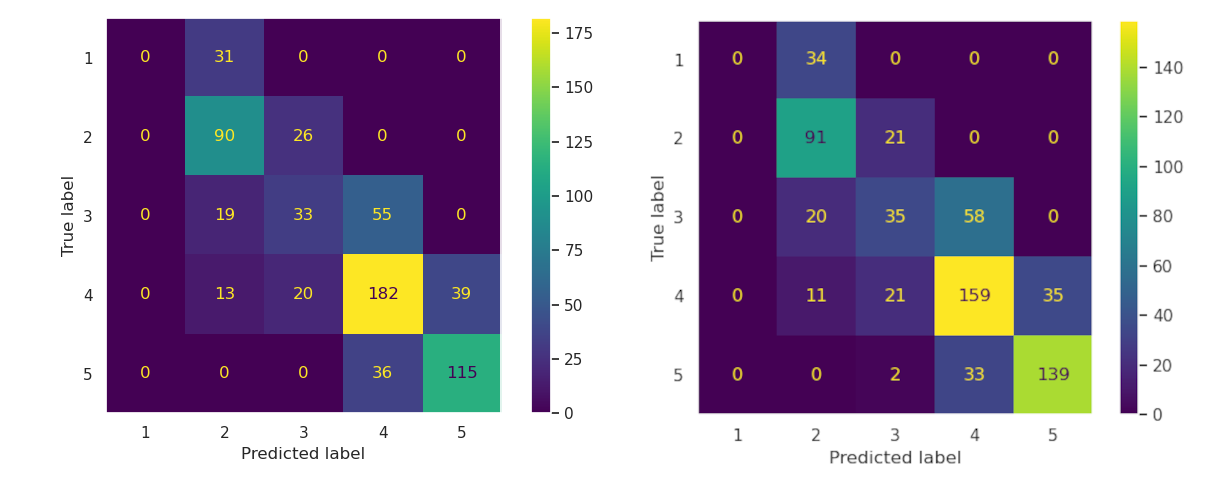
\includegraphics[width=0.95\linewidth]{confusion_matrices.png}\caption{Confusion matrices for decision tree (left) and neural net (right) classifiers.}
	\end{figure}
\end{frame}

%------------------------------------------------
\subsection{Conclusion}

\begin{frame}
    \frametitle{Summary}

    \begin{itemize}
	    \item Critical systems thinking is a general framework for systems thinking that encourages tailoring other approaches
	    \item On of those of sub-frameworks, Decision Intelligence (DI), is an especially powerful approach for mission-centric problem-solving
	    \item Using DI, we can create a causal decision diagram (CDD) as the basis of a decision model
	    \item Machine learning models and other assets support the links in the CDD, which can be converted into a ``digital twin'' if the benefits of doing so outweigh costs
	    \item We can use the resulting decision model as a collaborative and iterative approach for making complex, goal-directed decisions
    \end{itemize}
\end{frame}

%------------------------------------------------

\begin{frame} % Use [allowframebreaks] to allow automatic splitting across slides if the content is too long
	\frametitle{References}
	
	\begin{thebibliography}{99} % Beamer does not support BibTeX so references must be inserted manually as below, you may need to use multiple columns and/or reduce the font size further if you have many references
		\footnotesize % Reduce the font size in the bibliography
		
		\bibitem[Jackson, 2019]{p1}
			MC Jacson (2019)
			\newblock Critical Systems Thinking and the management of complexity
			\newblock \emph{Wiley}
			
		\bibitem[Pratt and Malcolm, 2023]{p2}
			LY Pratt and NE Malcom (2023)
			\newblock The Decision Intelligence handbook: practical steps for evidence-based decisions in a complex world
			\newblock \emph{O'Reilly}
	\end{thebibliography}
\end{frame}

%----------------------------------------------------------------------------------------
%	CLOSING SLIDE
%----------------------------------------------------------------------------------------

\begin{frame}[plain] % The optional argument 'plain' hides the headline and footline
	\begin{center}
		{\Huge The End}
		
		\bigskip\bigskip % Vertical whitespace
		
		{\LARGE Questions? Comments?}
	\end{center}
\end{frame}

%----------------------------------------------------------------------------------------

\end{document} 
